\documentclass[11pt]{article}
\usepackage[spanish]{babel}
\usepackage{graphicx}
\graphicspath{ {./imagenes/} }
\usepackage[section]{placeins}

\title{Proyecto \#2: Programación paralela\\
Algoritmo de Dijkstra\\
\large Estructura de datos y algoritmos II}

\author{Cabello, Sofía
\and López, Ricardo
\and Núñez, Diego}

\begin{document}

\maketitle{}

\section{Introducción}
El campo de la arquitectura digital de las computadores ha crecido exponencialmente en los últimos años. De manera simultánea, la investigación sobre diferentes formas de concurrencia, desde la segmentación estándar hasta paralelismo puro y la creación de estructuras que puedan soportar modelos de programación para estos sistemas han permito que la capacidad y productividad del hardware continue creciendo también. Los cumputadores modernos se vuelven cada vez más eficientes al contar con más procesadores, núcleos y memoria. Esta una tendencia que se espere que continue en los próximos años. 

\paragraph{}
La ventaja de esto es que múltiples procesadores pueden cumplir una tarea o pueden dividirla para que más de un hilo trabaje sobre ella, cuyo resultado óptimo sería ejecutarla en menos tiempo que si sólo se hiciera de manera secuencial. Una de las formas de medir este rendimiento es a través de la complejidad que tiene, en el caso de un algoritmo paralelo se mide por el tiempo y el número de procesadores que se requieren. EL nuevo reto es orientar el diseño computacional a la simplicidad y alto rendimiento, pero conservando un bajo costo y necesidad de poder, el paralelsimo juega un papel importante en esto. 

\paragraph{}
El problema de camino más corto es uno de los problemas fundamentales de optimización y uno de los más notorios en modelos computacionales paralelos debido a su amplio campo de aplicaciones. En este proyecto, abordarenos este problema haciendo uso del algoritmo de Dijkstra con la objetivo de analizar primero la definición y funcionaiento del algoritmo, tomando en cuenta sus características, psudocódigo, ventajas y analizando en particular la implementación paralela. Finalmente se hará una comparación entre las dos versiones para encontrar cuál resulta más eficiente al hacer pruebas con OpenMP en el lenguaje C. 
\section{Antecendentes}
Aunque hay una gran cantidad de estudios teóricos reportados sobre el procesamiento de grafos como Arjomandi en 1975 [], Benltey en 1980[], en el pasado no muchos de ellos consideraron el algoritmo para la ruta más corta. Uno de los pocos a encontrar fue realizado en 1980 por Deo et al. [] en el que se diseñó, codificó y se ejecutó un algoritmo paralelo en una computadora con arquitectura MIMD. 

\paragraph*{}
En los últimos 20 años, sin embargo, se ha explorado mucho más. Una de estas implementaciones fue realizada por Fang Zhou Lin y Nan Zhao [] en 1999. Respecto a aplicaciones, en 2012, Songmin Jia, Xiaolin Yin, y Xiuzhi Li [] propuesieron una técnica de Localización y Construcción de Mapas Simulánea (SLAM por sus siglas en inglés \textit {Simultaneous Localization and Map Building}) que resulta eficiente para la navegación de robots móbiles interiores basada en OpenMP. 
El código implementado para realizar las prubas fue tomado de...


\section{Programando en OpenMP}
OpenMP es una API (interfaz de programa de aplicación) que se utiliza para dirigir explícitamente el paralelismo de memoria compartida. OpenMP se introdujo en 1997 para estandarizar las extensiones de programación para máquinas de memoria compartida. OpenMP se ha convertido en el entorno elegido por muchos, de los practicantes de este tipo de programación. Consiste en un conjunto de directivas que se agregan al código C / C ++ / FORTRAN que manipula los subprocesos, sin que el programador tenga que lidiar con los subprocesos directamente. De esta manera obtenemos "lo mejor de ambos mundos": el verdadero paralelismo de los hilos (no preventivos) y el placer de evitar las molestias de la programación de hilos []. 

\paragraph{}
OpenMP proporciona una API "basada en directivas". Esto significa que hay instrucciones especiales de preprocesador conocidas como pragmas. Los pragmas generalmente se agregan a un sistema para permitir comportamientos que no son parte de la especificación C básica. Los compiladores que no apoyan los pragmas son libres de omitirlos. Esto permite que un programa que utiliza los pragmas se ejecute en cualquier plataforma. Entonces, en principio, si tiene un programa OpenMP cuidadosamente escrito, se puede compilar y ejecutar en cualquier sistema con un compilador C, independientemente de
si el compilador es compatible con OpenMP.

\paragraph{}
Esta directiva le dice al sistema de tiempo de ejecución que ejecute el siguiente bloque estructurado de codificar en paralelo. Puede bifurcar o iniciar varios subprocesos para ejecutar el bloque estructurado, que es un bloque de código con un único punto de entrada y una única salida. El número de subprocesos iniciados depende del sistema, pero la mayoría de los sistemas
comienza un hilo para cada núcleo disponible.

\paragraph{}
La ventaja de tener varios núcleos es que podríamos usar estos núcleos para extraer el paralelismo a nivel de subprocesos en un programa y, por lo tanto, aumentar el rendimiento de un solo programa. Se han realizado muchas investigaciones en esta área. Algunas de las ventajas de OpenMP incluyen: buen rendimiento, portátil (es compatible con una gran cantidad de compiladores), requiere muy poco esfuerzo de programación y permite que el programa ser paralelos incrementalmente.
\section{El algortimo de Dijsktra}
El algoritmo de Dijkstra es uno de los principales usados para encontrar las rutas más cortas en un gráfico ponderado por bordes y / o vértices. Dado un vértice de inicio en particular, encuentra el camino más corto desde todos los demás vértices del gráfico, incluido el destino deseado. 

\paragraph{}
Suponiendo que el camino más corto de s a t en la gráfica G pasa a través del nodo intermedio x. Es claro que esta ruta debe contener la ruta más corta de s - x como un prefijo, de lo contrario, podríamos acortar la ruta s - t usando el prefijo s - x. Por lo tanto tenemos que encontrar primero la ruta más corta de s a x antes de encontrar la más corta entre s y t. 

\paragraph{}
Este algoritmo procede a hacer ciclos en los que en cada uno de ellos calcula la ruta más corta de x a un nuevo vértice. Esto sugiere una estrategia dinámica. La ruta más corta de s a sí mimo es trivial a menos que hayan pesos negativos. Una vez que se determina la ruta a un nodo x, se checan todos los adyacentes a x para ver si hay un ,mejor camino desde s a un otro vértice atravesando a x.

\paragraph{}
Esto se puede explicar como referencia los siguientes pasos:

\begin{enumerate}
\item Seleccionar vértice de partida, es decir un origen.
\item Marcar el punto de partida como el punto de inicio.
\item Determinar los caminos especiales desde el nodo de partida, esdecir, el de inicio.
\item Camino especial es aquel que solo puede trazarse a través de los nodos o vértices ya marcados.
\item Para  cada  nodo  no  marcado,  se  debe  determinar  si  es  mejor  usar  el  camino  especial antes calculado o si es mejor usar el nuevo camino especial que resulte al marcar este nuevo nodo.
\item Para  seleccionar  un  nuevo  nodo  no  marcado  como  referencia,  deberá  tomarse  aquel cuyo camino especial para llegar a él es el mínimo, por ejemplo si anteriormente marqué el  nodo  o  vértice  2,  el  cual  tiene  dos  nodos  adyacentes  3  y  4  cuyo  peso  en  la  arista corresponde a 10 y 5 respectivamente, se tomará como nuevo nodo de partida el 4, ya que el peso de la arista o camino es menor.
\item Cada camino mínimo corresponde a la suma de los pesos de las aristas que forman el caminopara  ir  del  nodo  principal  al  resto  de  nodos,  pasando  únicamente  por  caminos especiales, es decir nodos marcados.
\end{enumerate}

\begin{figure}
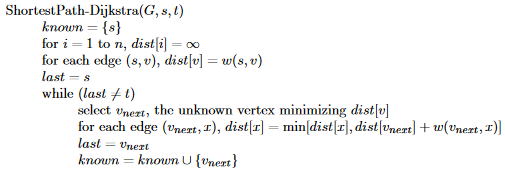
\includegraphics[width=0.9\linewidth]{algoritmo.png}
  \caption{Algoritmo de Dijstra.}
\end{figure}

\par
La complejidad del algoritmo de Dijkstra en su versión serial es de $O(n^2)$ si no se usa una cola de prioridad, como es el caso de las implementaciones realizadas para este proyecto. Es igualmente costos calcular la ruta más corta de un vértice s a cualquier otro vértice como lo es calcular la ruta más corta de cualquier vértice a s. Por esto, se puede decir que el nodo origen no afecta el rendimiento. 

\paragraph{}
Hay muchas aplicaciones para el algoritmo de Dijkstra, algunas de las más relevantes las podemos encontrar en los mapas, por ejemplo Google Maps u otros servicios de navegación. Una aplicación particularmente relevante es en la epidemiología. Una versión de este tipo de algoritmo puede ser usada en el cálculo del tamaño esperado del brote de un simple contagio en una red de contactos conocida, generalmente esta operación se lleva a cabo mediante una simulación computacionalmente intensiva que permite modelar todas las redes que cambian dinámicamente cuando el contagio solo puede viajar hacia adelante en el tiempo.



\section{Algoritmo utilizado y su implementación }

Primero que nada, es importante aclarar que nos basamos en código encontrado en (Matloff, 2012) con algunas modificaciones, ya que se generaba una condición de carrera que será explicada más adelante.
\par 
¿Cómo correr el programa? El programa recibe dos parámetros desde la terminal, uno para indicar el número de nodos que tendrá el grafo aleatorio (llamado nv dentro del programa) y otro para indicar si se deben imprimir los resultados. Aunque esta última opción parece un poco extra o tonta, fue muy útil para las pruebas de rendimiento.
\par 
El programa comienza llenando la matriz de adyacencia del grafo. Como el programa crea grafos ponderados bidireccionales, no se ingresan valores negativos a la matriz. Primero se llena una mitad y después los valores son copiados a la otra, ya que la matriz debe ser simétrica.
\par 
Después, se inicializan los valores de un arreglo de nv espacios que indica si un nodo todavía no ha sido visitado. Al nodo 0 le corresponde el espacio 0 de este arreglo, al 1 el espacio 1 y así sucesivamente hasta nv-1. Cuando existe un valor de 1, entonces el nodo todavía no ha sido visitado. A este arreglo se le conoce como no notDone.
\par
Junto al arreglo anterior se inicializan los valores de otro arreglo llamado mind, que almacena las distancias mínimas almacenadas hasta el momento hacia cada nodo. Por defecto, estas distancias se inicializan con el valor de la arista que conecta directamente a cualquier nodo con el nodo 0. Además, este arreglo almacena datos de tipo usigned, ya que esta versión del algoritmo que no utiliza una cola de prioridad no funciona con pesos negativos. 
\par
Teniendo todo listo comienza el algoritmo en sí. Se encuentra el constructor parallel, lo que significa que a partir de este punto se utilizarán varios hilos. Primero, se inicializan tres variables, step, mymv y mymd. La primera variable indica que nodo se está revisando en un momento. Cada nodo es revisado una vez, por esta razón step va desde 0 hasta nv-1. La segunda y la tercera sirven para almacenar de manera local para los hilos cual es el nodo más cercano al nodo inicial que han encontrado de manera individual. 
\par
Después, en un bloque single, se inicializa los valores de mv y md. Estas variables almacenan el nodo más cercano al nodo inicial de entre todos los encontrados por todos los hilos. La variable md se inicializa en -1 (Que, como las distancias son de tipo unsigned, en realidad representa el mayor entero posible) y mv en 0. Esto es así ya que la distancia mínima encontrar al inicio del algoritmo es presuntamente infinita y el vértice hacia el que hay esa distancia es presuntamente inexistente hasta que se indique lo contrario.
\par
Después, en una estructura omp for, cada hilo trabaja con un subconjunto de los nodos adyacentes al nodo 0, cada uno determina cual es el más cercano de su subconjunto. Luego, en una estructura critical, cada hilo pasa uno por uno a revisar si su menor valor encontrado es menor al ya existente. Si es así, se actualizan mv y md para referir al nodo más cercano en la iteración.
\par
En una estructura single, se marca a este nuevo nodo más cercano como revisado, así que en la siguiente iteración ya no podrá ser seleccionado como el nodo más cercano al inicial.
\par
Finalmente, en un ciclo for también paralelizado, se calculan distancias hacia todos los demás nodos y si es menor a la distancia más corta ya existente, se actualiza. 
\par
En este punto es donde se generaba la condición de carrera. OpenMP no asegura la manera ni el orden en cómo se ejecutarán las iteraciones de una estructura for. Por esta razón, un hilo podía terminar su parte primero y llegar a esta sección antes de que el otro, actualizando las distancias antes de que los demás hilos propusieran un nodo para ser el más pequeño en general. Para arreglar esto, se agregó una barrera después del critical, de esta manera se espera que todos los hilos actualicen mv y md si lo requieren antes de continuar. 
\par
En la siguiente iteración se repite el proceso, solo que esta vez ya estará marcado el nodo más cercano que se utilizó en la iteración anterior, por lo que ahora se ocupará el segundo más cercano y así sucesivamente hasta que no haya más nodos adyacentes al nodo inicial.


\begin{figure}[!htbp]
\centering
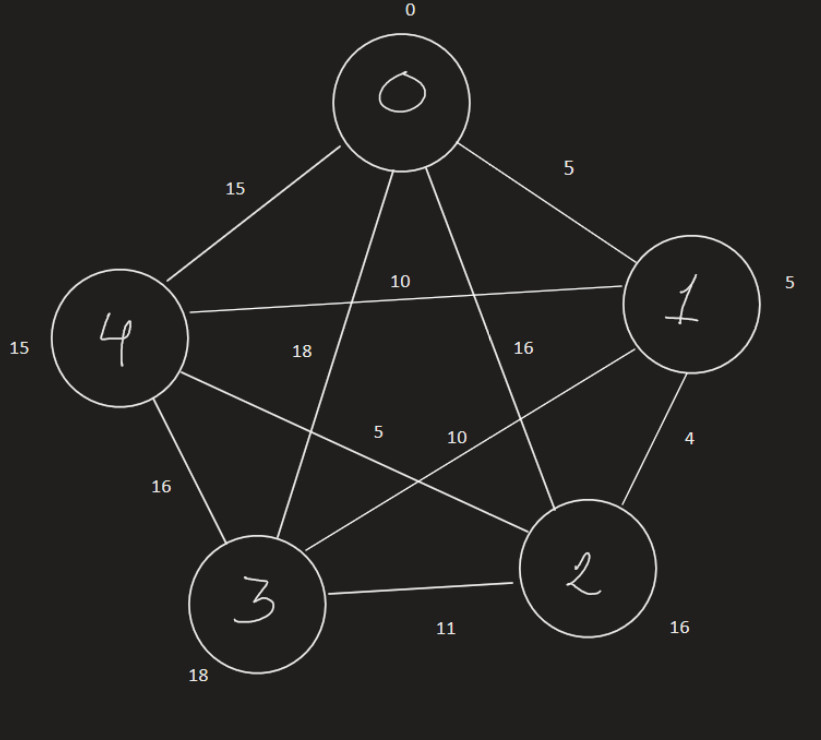
\includegraphics[scale = .5]{grafos1}
\caption{Grafo inicial}
\end{figure}

\begin{figure}[!htbp]
\centering
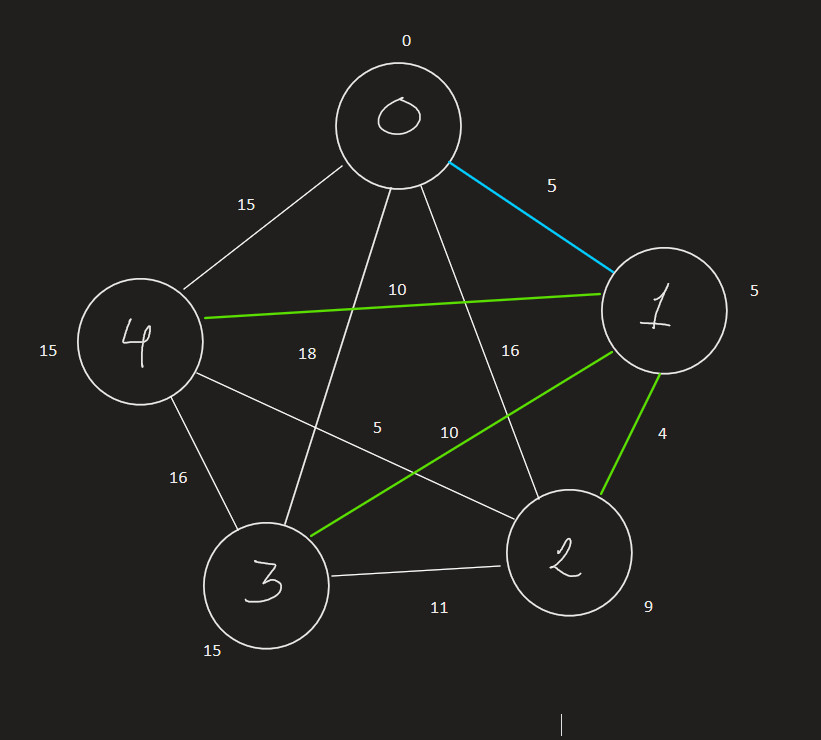
\includegraphics[scale = .5]{grafos2}
\caption{Primero se visita al nodo al nodo adyacente más cercano al origen.}
\end{figure}


\begin{figure}[!htbp]
\centering
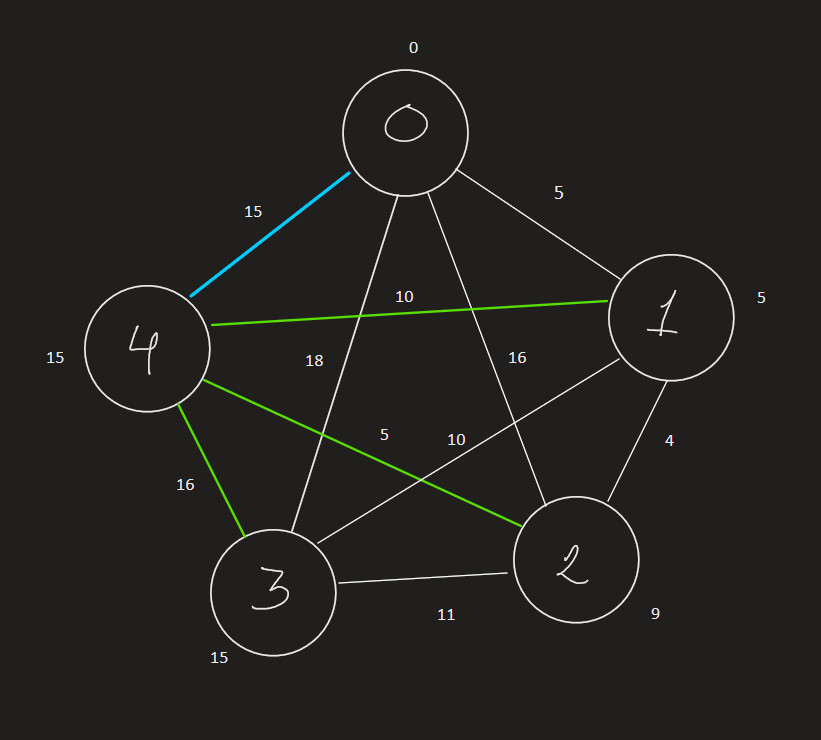
\includegraphics[scale = .5]{grafos3}
\caption{Después se visita el segundo más cerca.}
\end{figure}

\begin{figure}[!htbp]
\centering
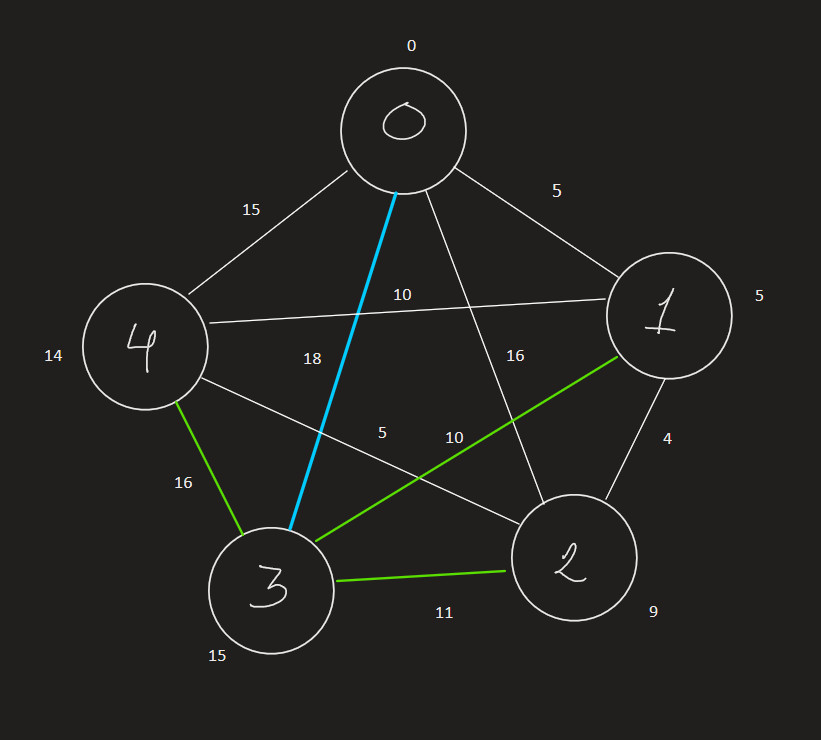
\includegraphics[scale = .5]{grafos5}
\caption{El algoritmo finaliza una vez que se visitó el más lejano.}
\end{figure}


\section{Pruebas}

\par
Se realizaron múltiples pruebas para analizar el rendimiento del programa. Para ellos fue necesario ejecutar en tres diferentes procesadores las diferentes versiones y analizar su comportamiento. 

\par
Empezaremos comparando a la versión paralela consigo misma. n la Figura 2 se puede ver que sin importar el procesador que se use, la tendencia es que al usar más hilos, aumenta el tiempo de ejecución del programa. Esto se hace más evidente dependiendo del número de núcleos con los que cuente la computadora.  

\begin{figure}[!h]
\centering
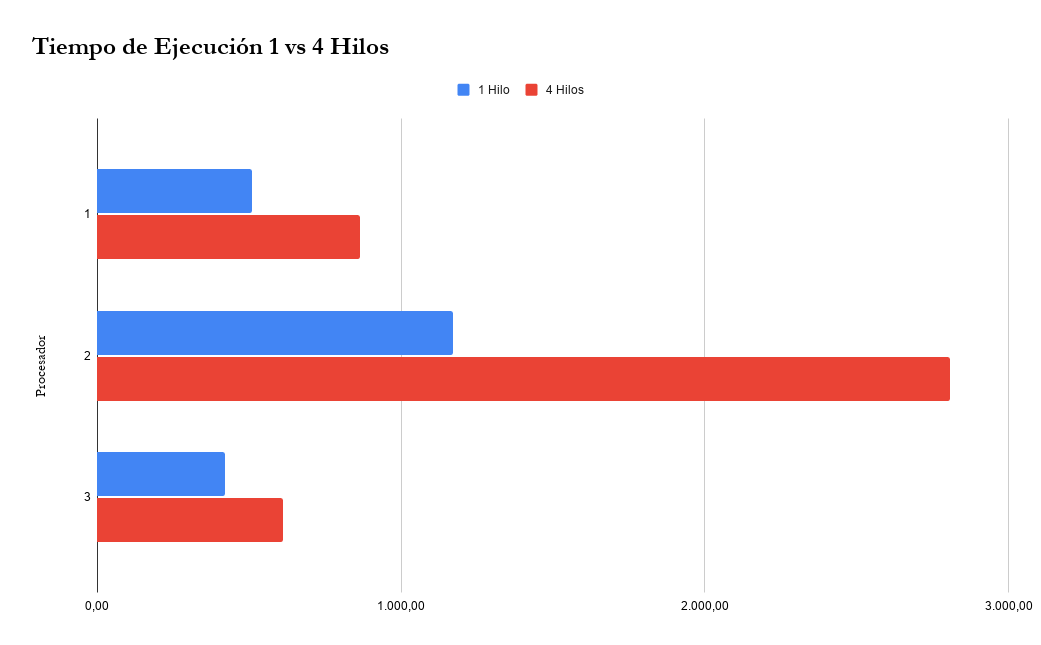
\includegraphics[width=0.9\linewidth]{hil1v4.png}
  \caption{Ejecución en segundos usando 3 diferentes procesadores.}
\end{figure}

\paragraph{}
Ahora, si comparamos el rendimiento de la versión serial contra la paralela (usando 4 hilos, es claro que el algoritmo linear es más eficiente. La diferencia crece conforme aumenta el tamaño de los datos. 

\begin{figure}[!h]
\centering
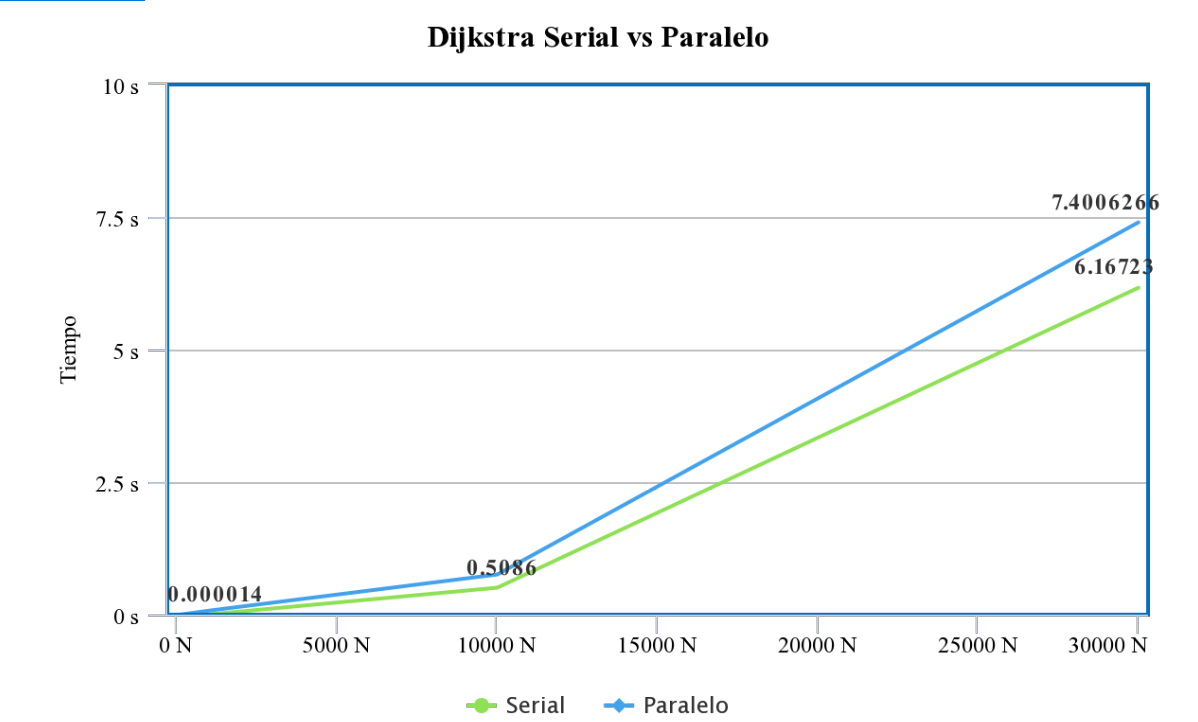
\includegraphics[width=0.9\linewidth]{svp.png}
  \caption{Rendimiento de programa serial vs paralelo.}
\end{figure}

\paragraph{}
En consecuencia, se puede decir que este algoritmo no es óptimo en su versión paralela. A pesar de segmentar las tareas entre hilos, la versión serial resulta ser la mejor opción. Algo importante a notar aquí es que esto fue probado en programa de OpenMP y que el lenguaje, así como API, de implementación juega un rol en el rendimiento final. Además, sería posible hacer modificaciones al código utilizado con el fin de hacer su ejecución más rápida.
\end{document}
